\begin{figure}[H]
    \centering
    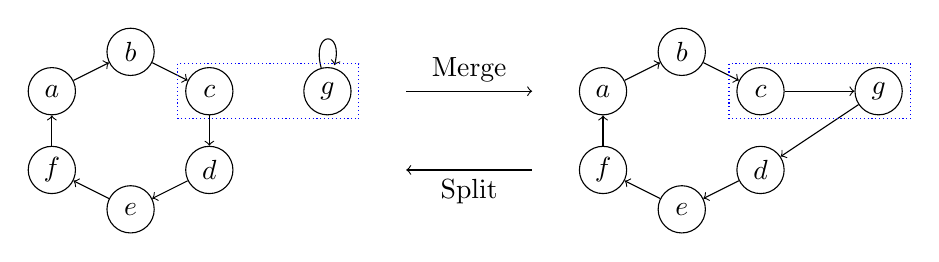
\begin{tikzpicture}[node distance=2cm, 
        outer/.style={circle,draw,inner sep=1pt, minimum size=6mm}
    ]
        % Left graph
        \node[outer] (a1) at ( -1.5, 3) [] {$a$};
        \node[outer] (f1) at ( -1.5, 2) [] {$f$};
        \node[outer] (b1) at ( -0.5, 3.5) [] {$b$};
        \node[outer] (c1) at (  0.5, 3) [] {$c$};
        \node[outer] (d1) at (  0.5, 2) [] {$d$};
        \node[outer] (e1) at ( -0.5, 1.5) [] {$e$};
        \node[outer] (g1) at (  2, 3) [] {$g$};
        
        % Edges
        \draw
            (a1) edge[->] (b1)
            (b1) edge[->] (c1)
            (c1) edge[->] (d1)
            (d1) edge[->] (e1)
            (e1) edge[->] (f1)
            (f1) edge[->] (a1)
            (g1) edge[loop above] (g1);
        
        \draw[densely dotted, blue] ( 0.1, 3.35) rectangle ( 2.4, 2.65);
        
        % Right graph
        \node[outer] (a2) at (  5.5, 3) [] {$a$};
        \node[outer] (f2) at (  5.5, 2) [] {$f$};
        \node[outer] (b2) at (  6.5, 3.5) [] {$b$};
        \node[outer] (c2) at (  7.5, 3) [] {$c$};
        \node[outer] (d2) at (  7.5, 2) [] {$d$};
        \node[outer] (e2) at (  6.5, 1.5) [] {$e$};
        \node[outer] (g2) at (  9, 3) [] {$g$};
        
        % Edges
        \draw
            (a2) edge[->] (b2)
            (b2) edge[->] (c2)
            (c2) edge[->] (g2)
            (d2) edge[->] (e2)
            (e2) edge[->] (f2)
            (f2) edge[->] (a2)
            (g2) edge[->] (d2);
        
        \draw[densely dotted, blue] ( 7.1, 3.35) rectangle ( 9.4, 2.65);
        
        \draw[->] (3,3) -- node[above] {Merge} (4.6,3);
        \draw[<-] (3,2) -- node[below] {Split} (4.6,2);

    \end{tikzpicture}
    \caption{
    Let $\graphG$ be a connected graph with seven vertices where edge $\createOrd{c,g}$ must exist in $\edgeFuncG$.
    The left image denotes the current configuration as directed cycles and the blue rectangle shows
    which swap will be applied to achieve the configuration on the right image.
    This operation \textit{merges} the two cycles and reapplying the swap returns the configuration to its original
    configuration, effectively \textit{splitting} the two cycles.
    }
    \label{img:mergesplit}
\end{figure}